%----------------------------------------------------------------------------------------
%	Header stuff that doesn't really matter...
%----------------------------------------------------------------------------------------
\documentclass[paper=letter, fontsize=11pt]{scrartcl}
\usepackage[T1]{fontenc}
\usepackage{fourier}
\usepackage[english]{babel}
\usepackage{amsmath,amsfonts,amsthm}
\usepackage{caption}
\usepackage{sectsty}
\usepackage{graphicx}
\usepackage{float}
\allsectionsfont{\normalfont\sffamily\bfseries}
\usepackage{fancyhdr}
\fancyhead[R]{Phil Crumm 804-005-575 | Connor Proctor 703-999-284}
\fancyfoot[L]{}
\fancyfoot[C]{}
\fancyfoot[R]{\thepage}
\renewcommand{\headrulewidth}{0pt}
\renewcommand{\footrulewidth}{0pt}
\setlength{\headheight}{13.6pt}

%----------------------------------------------------------------------------------------
%	Title area
%----------------------------------------------------------------------------------------

\newcommand{\horrule}[1]{\rule{\linewidth}{#1}}

\title{	
\normalfont \normalsize 
\textsc{University of California, Los Angeles} \\ [25pt]
\horrule{0.5pt} \\[0.4cm]
\Large Computer Science M152A - Digital Design Lab \\
\horrule{2pt} \\[0.5cm]
}

\author{Phillip Crumm \\*804-005-575 \\* Connor Proctor \\* 703-999-284 \\* \\*Lab 1: Laboratory Familiarization: The Real World}

\date{\normalsize January 16, 2014}
\usepackage[parfill]{parskip}
\begin{document}

\clearpage\maketitle
\thispagestyle{empty}
\pagebreak

%----------------------------------------------------------------------------------------
%	The body
%----------------------------------------------------------------------------------------

\section{Objective}
This laboratory's purpose is to familiarize ourselves with the hardware and tools that will be utilized for the duration of this course. Through a series of experiments, we explore several physical chips, breadboarding, circuit design, and the VHDL design language.

\section{Exercise 1 - TTL/CMOS Static Electrical Characteristics}
For this exercise, we explore the operating characters of TTL and CMOS NAND gates through the 74LS00 and 74HC00, respectively.

\subsection{74LS00 (TTL)}
First, we set IN to HI and receive output of LO, 0.1V. This is below the maximum $V_{OL}$ specified by datasheet and is a reasonable output. Second, we set IN to LO and receive output of HI, 4.9V, which is above the mimimum $V_{OH}$ specified by the datasheet. These results are reasonable.

\subsection{74HC00 (CMOS)}
We repeat the above using the 74HC00, and anticipate similar reuslts as they are bot NAND gates. First, we set IN to HI and receive LO output which is below $V_{OL}$ and thus acceptable. Next, we set IN to LO and receive HI, as expected. This is above $V_{OH}$ and not problematic.

\subsection{Interfacing TTL and CMOS}
Some difficulty occurs in interfacing TTL and CMOS gates. The CMOS gate, the 74HC00, designates LO as 0-0.5V and HI as 3.5V-15(!)V. On the other hand, the TTL gate, the 74LS00, sets LO As 0-.8V and HI as 2V-5V.

The CMOS gate is less noise sensitive and input-limited than the TTL gate; thus interfacing the two may cause some undesired results. When a TTL gate is connected to a CMOS gate, the circuit behaves as expected; the TTL gate's output is within the noisy margin of the CMOS gate. On the other hand, when the CMOS gate is connected to the TTL gate, LO is output consistently. This is because the CMOS gate's output is not within the tight margins required by the TTL gate.

\section{Exercise 2 - 555 Timer}
For the second exercise, we configure a 555 Timer and evaluate its use as a clock. After configuring the timer with two 10k resistors and one 10nF capacitor, we measure the output (pin 3) of the timer. We measure the frequency to approximate as 1/150 cycles per microseconds (for a period of 150 microseconds); this is equal to 6600Hz. Total time spent HI is 100 microseconds, leading to a duty cycle of 66\%.

We then replace the second resistor in the series, $R_{1}$, with a 1-10k variable potentiometer. We adjust the knob to find a duty cycle of about 60\%. As we adjust the potentiometer, time spent HI is increased; time spent LO is unchanged. We eventually settle on slightly above 50\%, or 5k resistence, for a duty cycle of 60\%.

The contionus, predictible, and periodic behavior of the wave makes it effectively used as a clock. Its datasheet confirms its relatively accurate timing stability and margin of error (within 1\%). We find the clock to output nearly 5V on every HI cycle, which is suitably HI enough for any other chips we have thus far encountered.

\section{Exercise 3 - Glitches}
This glitch is a consequence of the propagation delay between each NAND gate; for a brief period of time, CLK will output the opposite of output 11 (the third NAND gate in the three-gate inverter series) due to the delay. This glitch is not measurable as it is quite small--further, its length varies with each oscillation.

\section{Exercise 4 - Asynchronous Counter}
Next, we configured the asynchronous counter using the 74LS393 as shown. After configuration, we measure the output of the clock to verify its accuracy. Starting from the least significant bit, we note that the time spent LO and HI (the period) increase by a power of two for each bit, as we would expect a binary-counting clock to behave.

\section{Exercise 5 - Synchronous Counter}
Continuing on, we connected two synchronous counter (74LS163). For consistency, we connected the click output to inputs 2 on both counters. We then utilized the scope determine that each counter was operating as desired. The first counter increments always; the second, only when the first has reached its overflow.

This is consistent with our understanding of the operation of the T input and RCO output. The T input acts as an enabler bit for the counter; the counter will count up if and only if T is HI. This is consistent with our observations; the first counter, with T to HI counts always; the second, with T to the first counter's RCO outputs if and only if T has reached its maximum.

The RCO output, or ripple-carry output, is LO unless the current counter is overflowing; it then fires HI.

Both the asynchronous 74LS393 and the synchronous 74LS163 will require four flip-flops per output bit to maintain state. The synchronous 74LS163 will also require additional circuitry to enable synchronous operation (ensuring it operates only when the equivalant of T is enabled), increasing the complexity. Depending on additional hardware available, this may be a trivial increase to the 8 bits of flip-flops required to maintain state.

\section{Exercise 6 - Ring Oscillator}
You can create a ring oscillator by chaining an odd number of inverter gates together. Doing this creates an oscillator because of propogation delays within each gate. After the input to a gate has changed, it takes an amount of time for the output to change accordingly. Since we are using an odd number of gates, the output of the last gate is the opposite of the first gate. So once the signal has propagted through all the gates, the input to the first gate changes and the process starts over. (Note that the "first" gate can be any arbitrary gate in the chain.) This affect can be seen in the timing diagram below.
\begin{figure}[H]
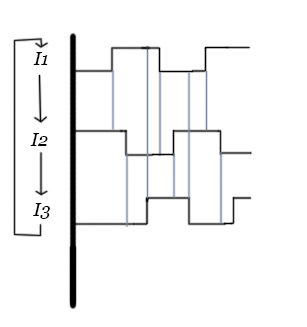
\includegraphics[height=75mm]{timing_diagram.png}
\centering
\caption{Three inveter timing diagram}
\label{overflow}
\end{figure}
\subsection{11 Gate Ring Oscillator}
We first used two hex inverter chips (74LS04) to chain 11 inverter gates together in a loop.
After we verified that this ring oscillator was working, we then measured the period of oscillation to be 0.12 microseconds. By taking the half-period and dividing it by the number of gates, we can determine an average propogation delay per gate of about 0.0055 microseconds. One over the period gives us a frequency of 8.33 oscillations/microsecond. The 11 gate oscillator had a maximum of 2.2 volts and a minimum of 1.5 volts.
\subsection{17 Gate Ring Oscillator}
Next we wired up another 6 more inverters into the circuit for a total of 17. Based on the propogation delay of the gates measured in the previous exersize, the period of oscillation for 17 gates should be 2*17*0.0055 = 0.187 microseconds. Using the oscilloscope, we meassured the period to be 0.19 microseconds, surprisingly close to the calculated value! The minimum and maximum voltages we measured to be 1 and 5 volts, respectively. This is a lot cleaner than the 11 gate oscillator, possibly due to the period being longer giving the voltage more time to equalize. 

\section{Exercise 7 - Set-Reset Latch with NAND Gates}
A (non-gated) SR latch has two inputs, S (set) and R (reset), and two outputs (Q and Q'). When S is high (and R is low), Q goes high. Then after both S goes back to low, Q still stays "latched" high until R goes high. When R goes high, Q goes back to low and Q' goes high. It then "latches" like this until again S is pressed. We use two NAND gates and two inverters to achieve this. If both S and R are high (which is invalid input), then both Q and Q' will go high. A gated SR latch uses two NAND gates in place of the inverter, with the 2nd input to these NAND gates hooked up to a new E (enable) input. When E is low, the S and R inputs cannot affect the main SR latch. Only when E is high is input enabled. We built a gated SR latch using 74LS00 chips, and it worked as expected.

\section{Exercise 8 - Writing Combinational VHDL Code}
We started by making Karnaugh Maps for each segment of the 7-segment display (see attached pre-lab). We then used this to program the logic of the FPGA (see attached code). The display has common anode, meaning that when we turned an individual segment low it turned on, and when high it turned off.

%----------------------------------------------------------------------------------------

\end{document}